\documentclass[tikz, border=5mm]{standalone}
\usepackage{tikz}
\usetikzlibrary{arrows.meta, positioning, calc}

\begin{document}

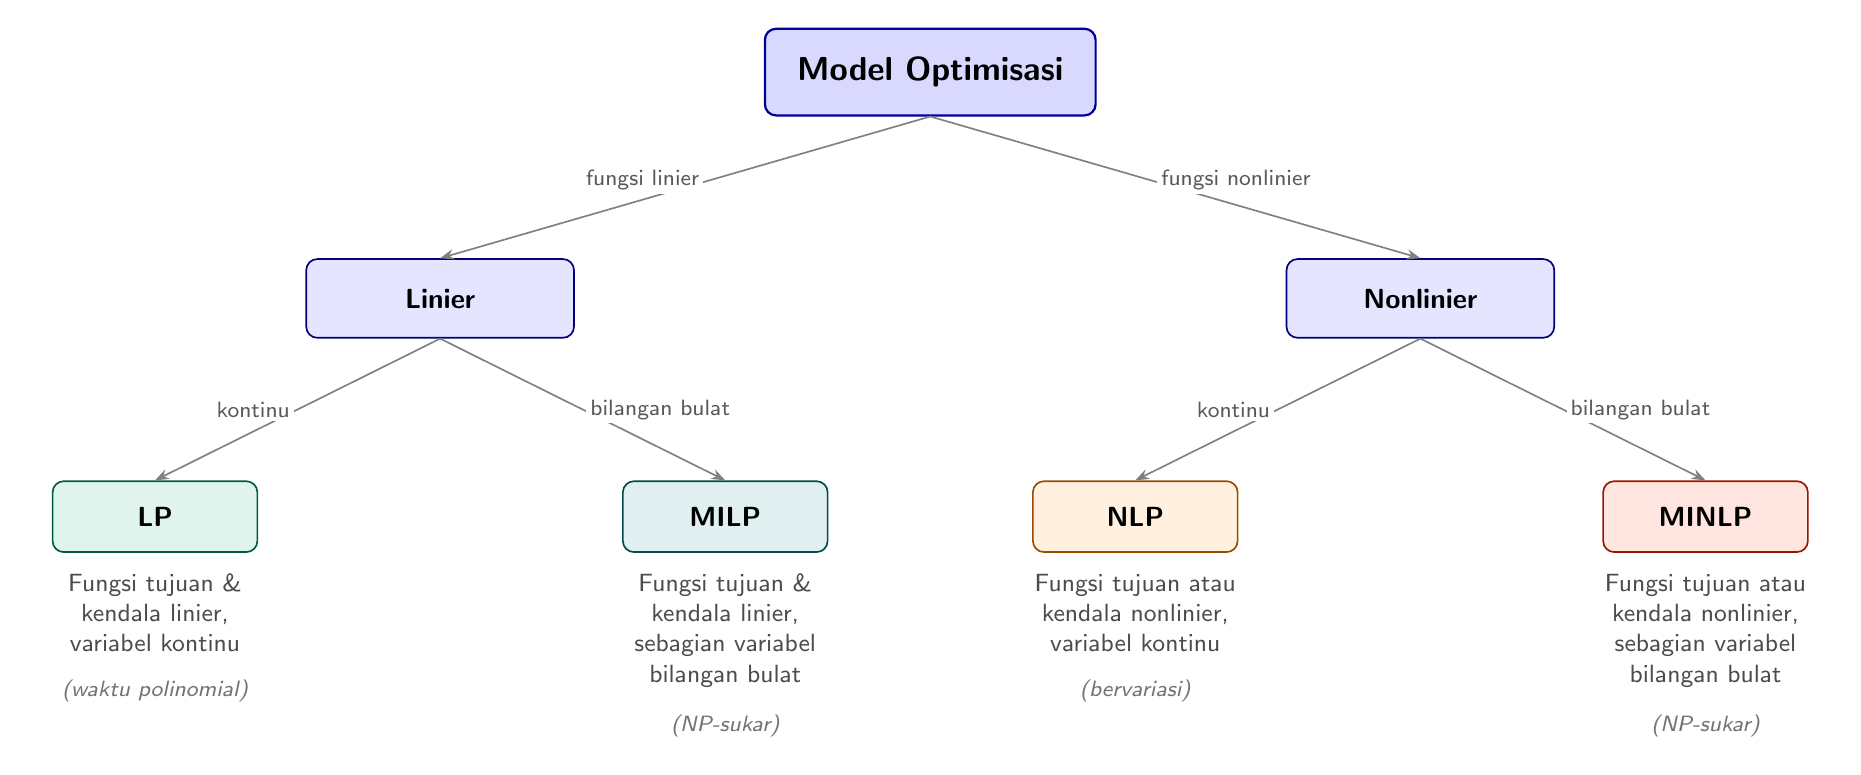
\begin{tikzpicture}[
    % Node styles
    root/.style={
        rectangle, rounded corners=4pt,
        minimum width=4.2cm, minimum height=1.1cm,
        text centered, font=\sffamily\bfseries\large,
        draw=blue!60!black, line width=0.8pt,
        fill=blue!15,
    },
    mid/.style={
        rectangle, rounded corners=4pt,
        minimum width=3.4cm, minimum height=1cm,
        text centered, font=\sffamily\bfseries,
        draw=blue!50!black, line width=0.6pt,
        fill=blue!10,
    },
    leaf/.style={
        rectangle, rounded corners=4pt,
        minimum width=2.6cm, minimum height=0.9cm,
        text centered, font=\sffamily\bfseries,
        draw=#1!60!black, line width=0.6pt,
        fill=#1!12,
    },
    leaf/.default=blue,
    desc/.style={
        font=\sffamily\small, text=black!70,
        text width=3.0cm, align=center,
    },
    complexity/.style={
        font=\sffamily\footnotesize\itshape, text=black!55,
    },
    edge label/.style={
        font=\sffamily\footnotesize, text=black!65,
        midway, fill=white, inner sep=1.5pt,
    },
    line/.style={
        draw=black!50, line width=0.6pt, -{Stealth[length=5pt]},
    },
]

% === Root ===
\node[root] (opt) {Model Optimisasi};

% === Level 2: Linear vs Nonlinear ===
\node[mid] (lin)    [below left=1.8cm and 2.4cm of opt]  {Linier};
\node[mid] (nonlin) [below right=1.8cm and 2.4cm of opt] {Nonlinier};

% === Level 3: The four problem classes ===
\node[leaf=green!60!blue] (lp)    [below left=1.8cm and 0.6cm of lin]    {LP};
\node[leaf=teal]          (milp)  [below right=1.8cm and 0.6cm of lin]   {MILP};
\node[leaf=orange]        (nlp)   [below left=1.8cm and 0.6cm of nonlin] {NLP};
\node[leaf=red!70!orange] (minlp) [below right=1.8cm and 0.6cm of nonlin]{MINLP};

% === Descriptions under leaves ===
\node[desc, below=4pt of lp]    (desc-lp) {Fungsi tujuan \&\\kendala linier,\\variabel kontinu};
\node[desc, below=4pt of milp]  (desc-milp) {Fungsi tujuan \&\\kendala linier,\\sebagian variabel bilangan bulat};
\node[desc, below=4pt of nlp]   (desc-nlp) {Fungsi tujuan atau\\kendala nonlinier,\\variabel kontinu};
\node[desc, below=4pt of minlp] (desc-minlp) {Fungsi tujuan atau\\kendala nonlinier,\\sebagian variabel bilangan bulat};

% === Complexity annotations ===
\node[complexity, below=3pt of desc-lp]    {(waktu polinomial)};
\node[complexity, below=3pt of desc-milp]  {(NP-sukar)};
\node[complexity, below=3pt of desc-nlp]   {(bervariasi)};
\node[complexity, below=3pt of desc-minlp] {(NP-sukar)};

% === Edges: root to level 2 ===
\draw[line] (opt.south) -- (lin.north)
    node[edge label, pos=0.45, left=2pt] {fungsi linier};
\draw[line] (opt.south) -- (nonlin.north)
    node[edge label, pos=0.45, right=2pt] {fungsi nonlinier};

% === Edges: level 2 to level 3 ===
\draw[line] (lin.south) -- (lp.north)
    node[edge label, pos=0.5, left=1pt] {kontinu};
\draw[line] (lin.south) -- (milp.north)
    node[edge label, pos=0.5, right=1pt] {bilangan bulat};
\draw[line] (nonlin.south) -- (nlp.north)
    node[edge label, pos=0.5, left=1pt] {kontinu};
\draw[line] (nonlin.south) -- (minlp.north)
    node[edge label, pos=0.5, right=1pt] {bilangan bulat};

\end{tikzpicture}

\end{document}
